\section{Methods for numerical calculations}
\label{sec:nft_numerical}

\subsection{Boffetta-Osborne method for determining scattering data}

This method was proposed in 1992 by Boffetta and Osborne and described in detail in their work \cite{osborne1992}. The main idea of the method is that the ZS system can be rewritten as:
\begin{equation}
    \left\{
    \begin{aligned}
        \partial_{t} \psi_1 = & - \xi \psi_1 + q \psi_2 \\
        \partial_{t} \psi_2 = & \sigma q^{*} \psi_1 + \xi \psi_2 \\
    \end{aligned}
    \right.
\end{equation}
which, after passing to a discrete grid for $ t $ variable, gives an evolution of the spectral eigenfunction $ \Psi $ on each interval $ \Delta t $:
\begin{equation}
    \Psi(t_n+\Delta t) = U(q_n)\Psi(t_n)
    \label{eq:bo_prop_0}
\end{equation}
where $ U (q_n, \Delta t) $ is represented as an exponential function of the matrix $ Q (\xi) $:
\begin{equation}
    U(q)=\mathrm{exp} [\Delta t Q(\xi)] = \mathrm{exp} \left( \Delta t
    \begin{pmatrix}
        -i \xi & q \\
        \sigma q^{*} & i \xi \\
    \end{pmatrix} \right)
    \label{eq:bo_prop_1}
\end{equation}

If we expand the above exponent into a Taylor series and sum up the matrices, and then, assuming that each element of the matrix is a Taylor series, we summarize these rows for each element, then we get the following expression for the propagator:
\begin{equation}
    \begin{aligned}
        U(q) & = \mathrm{exp}[\Delta t Q(\xi)] = \\
        & =
        \begin{pmatrix}
            \cosh(k \Delta x) - \frac{i \xi}{k}\sinh(k \Delta x) & \frac{q}{k}\sinh(k \Delta x) \\
            \frac{\sigma q^{*}}{k}\sinh(k \Delta x) & \cosh(k \Delta x) + \frac{i \xi}{k}\sinh(k \Delta x) \\
        \end{pmatrix}
    \end{aligned}
    \label{eq:bo_prop_2}
\end{equation}
where $ k^2 = \sigma | q |^2 - \xi^2 $ is a constant on the interval $ \Delta t $. Using the above method, we can solve the scattering problem --- determine the coefficients $ a (\xi) $ and $ b (\xi) $. However, for a discrete spectrum, this is not sufficient: since the coefficient $ a (\xi) $ is zero, it is necessary to calculate its derivative $ a'(\xi_n) = \frac{\partial a (\xi)} {\partial \xi} |_{\xi = \xi_n} $. Now we introduce a four-component field containing both the vector function $ \Psi $ and its derivative with respect to $ \xi $:
\begin{equation}
    \Xi(t, \xi) = 
    \begin{pmatrix}
        \Psi \\
        \Psi' \\
    \end{pmatrix}
\end{equation}
where $\Psi' = \partial \Psi / \partial \xi$. 
Similar to the expressions~(\ref{eq:bo_prop_1}) and (\ref{eq:bo_prop_2}) for the $ \Xi $ field, one can write a recursive relation by differentiating the expression~(\ref{eq:bo_prop_0}):
\begin{equation}
    \Xi(t_n + \Delta t) = T(q_n) \Xi(t_n)
\end{equation}
here 
\begin{equation}
    T(q_n) = 
    \begin{pmatrix}
        U(q_n) & 0 \\
        U'(q_n) & U(q_n) \\
    \end{pmatrix}
\end{equation}
$4 \times 4$ matrix, $U'(q_n) = \partial U(q_n) / \partial \xi$ and can be written as:
%\begin{equation}
%    \begin{pmatrix}
%        i \Delta t \frac{\xi^2}{k^2} \cosh(k \Delta t) - \left( \xi \Delta t + i + i \frac{\xi^2}{k^2} \right) \frac{\sinh (k \Delta t)}{k} & -\frac{q\xi}{k^2} \left( \Delta t \cosh(k\Delta t) - \frac{\sinh(k \Delta t)}{k}\right) \\
%        -\frac{\sigma q \xi}{k^2} \left( \Delta t \cosh(k\Delta t) - \frac{\sinh(k \Delta t)}{k}\right) & -i \Delta t \frac{\xi^2}{k^2} \cosh(k \Delta t) - \left( \xi \Delta t - i - i \frac{\xi^2}{k^2} \right) \frac{\sinh (k \Delta t)}{k} \\
%    \end{pmatrix}
%\end{equation}
\begin{eqnarray}
    U'_{11} = i \Delta t \frac{\xi^2}{k^2} \cosh(k \Delta t) - \left( \xi \Delta t + i + i \frac{\xi^2}{k^2} \right) \frac{\sinh (k \Delta t)}{k} \nonumber \\
    U'_{12} = -\frac{q\xi}{k^2} \left( \Delta t \cosh(k\Delta t) - \frac{\sinh(k \Delta t)}{k}\right) \nonumber \\
    U'_{21} = -\frac{\sigma q \xi}{k^2} \left( \Delta t \cosh(k\Delta t) - \frac{\sinh(k \Delta t)}{k}\right) \nonumber \\ 
    U'_{22} = -i \Delta t \frac{\xi^2}{k^2} \cosh(k \Delta t) - \left( \xi \Delta t - i - i \frac{\xi^2}{k^2} \right) \frac{\sinh (k \Delta t)}{k}
\end{eqnarray}
%\begin{equation}
%    \begin{aligned}
%        i \Delta t \frac{\xi^2}{k^2} \cosh(k \Delta t) - \left( \xi \Delta t + i + i \frac{\xi^2}{k^2} \right) \frac{\sinh (k \Delta t)}{k} & -\frac{q\xi}{k^2} \left( \Delta t \cosh(k\Delta t) - \frac{\sinh(k \Delta t)}{k}\right) \\
%        -\frac{\sigma q \xi}{k^2} \left( \Delta t \cosh(k\Delta t) - \frac{\sinh(k \Delta t)}{k}\right) & -i \Delta t \frac{\xi^2}{k^2} \cosh(k \Delta t) - \left( \xi \Delta t - i - i \frac{\xi^2}{k^2} \right) \frac{\sinh (k \Delta t)}{k} \\
%    \end{aligned}
%\end{equation}

For the numerical calculation, we consider the initial potential of $ q (t, 0) $ on the $ M + 1 $ segments, assuming that
\begin{equation}
    q(t, 0) = q_n  \quad \text{when} \quad t \in \left(t_n - \frac{\Delta t}{2}; \ t_n + \frac{\Delta t}{2} \right] {.}
\end{equation}
In this case, the discrete solution of the scattering problem is the following:
\begin{equation}
    \Xi(t_n) = \prod^{-M/2}_{j = n-1} T(q_j) \Xi(t_{-M/2}) {.}
\end{equation}

To obtain the scattering data, it is necessary to calculate the scattering matrix $ S $
\begin{equation}
    S(\xi) = \prod^{-M/2}_{j = M/2-1} T(q_j) = 
    \begin{pmatrix}
        \Sigma(\xi) & 0 \\
        \Sigma^{'}(\xi) & \Sigma(\xi) \\
    \end{pmatrix} {,}
\end{equation}
where matrix $\Sigma$ is defined as 
\begin{equation}
    \Sigma = \prod_{j = M/2-1}^{-M/2} U(q_j) {,} \quad 
    \Sigma^{'} = \partial \Sigma / \partial \xi {.}
\end{equation}

Initially, in the problem~(\ref{eq:ZS}), the vector function $ \Psi $ extended from $ -\infty$ to $ + \infty $. In numerical simulation, this interval is replaced by the interval from $ - \frac{T}{2} $ to $ +\frac{T}{2}$. In this case, we get the following result:
% \begin{equation}
%     \begin{aligned}
%         a(\xi) & = & S_{11}(\xi) e^{i\xi T} {,} \\
%         b(\xi) & = & S_{21}(\xi) {,}  \\ 
%         \frac{\partial a(\xi)}{\partial \xi} & = & [S_{31} + i \frac{T}{2} 
%             (S_{11} + S_{33})]e^{i\xi T } {,} \\
%         \frac{\partial b(\xi)}{\partial \xi} & = & S_{41} + i\frac{T}{2} (S_{43} - S_{21}) {.}
%     \label{eq:bo_result}
%     \end{aligned}
% \end{equation}
\begin{eqnarray}
    a(\xi) & = & S_{11}(\xi) e^{i\xi T} {,} \nonumber \\
    b(\xi) & = & S_{21}(\xi) {,}  \nonumber \\ 
    \frac{\partial a(\xi)}{\partial \xi} & = & [S_{31} + i \frac{T}{2} 
        (S_{11} + S_{33})]e^{i\xi T } {,} \nonumber \\
    \frac{\partial b(\xi)}{\partial \xi} & = & S_{41} + i\frac{T}{2} (S_{43} - S_{21}) {.} 
    \label{eq:bo_result}
\end{eqnarray}

This method allows us to find all the scattering data for an arbitrary $ \xi $. Although the method does not directly calculate the spectrum of the problem~(\ref{eq:ZS}), it can help us find it, because we know that at the points of the discrete spectrum on the complex plane the scattering coefficient $a (\xi) \equiv 0 $.

It should be noted that for $ t \ll 1 $ the matrix $ U (q) $~\ref{eq:bo_prop_2} reduces to
\begin{equation}
    U(q) \approx
    \begin{pmatrix}
        1 - i\xi \Delta t & q \Delta t \\
        \sigma q^{*} \Delta t & 1 + i \xi \Delta t \\
    \end{pmatrix} {.}
\end{equation}
This form was found by Ablowitz and Ladik \cite{ablowitz1975, ablowitz1976} and can also be used to solve the Zakharov-Shabat problem.


\subsection{T\"oplitz inner bordering method}

The formation of technologies for creating \acrlong{fbg}s (\acrshort{fbg}s) \cite{agrawal2002, kashyap1999} was accompanied by the development of numerical methods for their modeling and analysis. Recovery of the refractive index from a given dependence of the scattering coefficient on the frequency is the inverse scattering problem, which is solved in mathematical physics using a pair of \acrlong{glm} \cite{zakharov1972exact} equations.

The work \cite{belai2007} was proposed a method for solving the \acrshort{glm} equations (\ref{eq:glm_1}) and (\ref{eq:glm_2}). It consists in the fact that the \acrshort{glm} equations can be reduced to equations with the Toeplitz kernel by replacing $u(t,x) = A_1(t,t-x)$ and $v(t,y) = -A^{*}_2(t,y-t)$:
\begin{eqnarray}
    u(t,x)+\int_{x}^{2t} \Omega^{*}(y-x) v(t,y) dy = 0 \nonumber \\
    v(t,y)+\int_{0}^{y} \Omega(y-x) u(t,x) dx + \Omega(y) = 0
    \label{eq:glm_tib}
\end{eqnarray}
where $\Omega = \Omega_{sol} + \Omega_{rad} =  \sum_{n} c_n e^{-i \xi_n x} +
\frac{1}{2\pi} \int_{-\infty}^{+\infty} d\xi r(\xi) e^{-i \xi x}$ --- integral kernel, 
the parameters $ x $ and $ y $ are in the range $ 0 \leq x {,} y <2t $, the variable $ t $ is in the range $ 0 \leq t <T $, and the signal is restored using the formula $ q (t) = 2 v (t, 2t-0) $.

Further, the equations~(\ref{eq:glm_tib}) are discretized on a uniform grid, and the integrals are represented as sums.
The resulting equations have a block structure and are written in matrix form:
\begin{equation}
    \mathbf{G}
    \begin{pmatrix}
        \mathbf{u} \\
        \mathbf{v} \\
    \end{pmatrix} =
    \begin{pmatrix}
        \mathbf{a} \\
        \mathbf{b} \\
    \end{pmatrix}
\end{equation}
where matrix $\mathbf{G}$ and vectors $\mathbf{u}$, $\mathbf{v}$, $\mathbf{a}$ and $\mathbf{b}$
are defined by:
\begin{eqnarray}
    \mathbf{G} = 
    \begin{pmatrix}
        \mathbf{E} & \pm \mathbf{\Omega}^{\dagger} \\
        \mathbf{\Omega} & \mathbf{E} \\
    \end{pmatrix} {,}
    \quad
    \mathbf{\Omega} = h
    \begin{pmatrix}
        \frac{1}{2} \Omega_0 & 0 & \dots & 0 \\
        \Omega_1 & \frac{1}{2} \Omega_0 & \dots & 0 \\
        & & \ddots & \\
        \Omega_{m-1} & \Omega_{m-2} & \dots & \frac{1}{2} \Omega_0 \\
    \end{pmatrix} 
    \nonumber \\ 
    \mathbf{a} = \pm \frac{h}{2} v_m^{(m)} \tilde{\mathbf{\rho}^{*}} {,}
    \mathbf{b} = - \left( 1 + \frac{h}{2} u_1^{(m)} \mathbf{\rho} \right) {,} 
    \nonumber \\
    \mathbf{\rho} = 
    \begin{pmatrix}
        \Omega_1 \\
        \vdots \\
        \Omega_m \\
    \end{pmatrix} {,}
    \mathbf{u} = 
    \begin{pmatrix}
        u_1^{(m)} \\
        \vdots \\
        u_m^{(m)} \\
    \end{pmatrix} {,}
    \mathbf{v} =
    \begin{pmatrix}
        v_1^{(m)} \\
        \vdots \\
        v_m^{(m)} \\
    \end{pmatrix} {.}
\end{eqnarray}
$\mathbf{E}$ --- identity matrix.

The first and last elements of the solution vector are calculated by the formulas:
\begin{eqnarray}
    u_1^{(m)} = \pm \frac{h}{2} v_m^{(m)} \langle \mathbf{y}^{*} | \tilde{\mathbf{\rho}}^{*} \rangle
    \mp \left( 1 + \frac{h}{2} u_1^{(m)} \right) \langle \mathbf{z}^{*} | \mathbf{\rho} \rangle
    {,} \nonumber \\
    u_1^{(m)} = \pm \frac{h}{2} v_m^{(m)} \langle \tilde{\mathbf{z}} | \tilde{\mathbf{\rho}}^{*} \rangle
    - \left( 1 + \frac{h}{2} u_1^{(m)} \right) \langle \tilde{\mathbf{y}} | \mathbf{\rho} \rangle
    {.}
    \label{eq:tib_solution_vec}
\end{eqnarray}
Parentheses denote scalar product
$ \langle \mathbf{x} | \mathbf{y} \rangle = \mathbf{x}^{T} \cdot \mathbf{y} $.
We can introduce the following parameters
\begin{equation}
    \alpha_m = h \langle \mathbf{z}^{*} | \mathbf{\rho} \rangle {,} \quad
    \beta_m = h \langle \tilde{\mathbf{y}} | \mathbf{\rho} \rangle {.}
\end{equation}
Then equation~(\ref{eq:tib_solution_vec}) allows calculate $v^{(m)}_{m}$:
\begin{equation}
    v_m^{(m)} = \frac{ -\beta_m / h}
    {1 \pm \mathrm{Im} \ \alpha_m - \frac{1}{4}(|\alpha_m|^2 \mp |\beta_m|^2)} {.}
\end{equation}
We assume that with the required accuracy $ \alpha_m = -u (x_m, 0) h + O (h^2) $, which leads us to the final solution:
\begin{equation}
    q_m = 2 v_{m}^{(m)} = -2 \beta_m / h + O(h^2) {.}
\end{equation}

This procedure can be described as an algorithm that can be reversed. Next, we present two algorithms of direct and inverse transformations, as a result of which a signal can be reconstructed from the core (Algorithm~\ref{alg:itib}) and vice versa: the integral core is obtained from the signal (Algorithm~\ref{alg:dtib}).
\begin{algorithm}
    \caption{Inverse TIB algorithm for signal recovery from the kernel}
\label{alg:itib}
\begin{algorithmic}[1]

    \State $ m = 1 $ 
    $q_0 = -2\Omega_0 $
    $y_0^{(1)} = \frac{1}{1 \mp h^2 |\Omega_0|^2 / 4}$
    $ z_0^{(1)} = -\frac{y_0^{1} h \Omega_0}{2}$
    
    \State $ \beta_m = h \sum_{j=0}^{m-1}\Omega_{m-j} y_{j}^{(m)} $
    \State $ q_m = -2 \beta_m / h $

	\State $c_m = \frac{1}{1 \mp |\beta_m|^2}, d_m = -\beta_m c_m$

	\State $\mathbf y^{(m+1)} = 
		c_m \begin{pmatrix} \mathbf y^{(m)} \\ 0 \\ \end{pmatrix} +
		d_m \begin{pmatrix} 0 \\ \pm \mathbf{\tilde z}^{*(m)} \\ \end{pmatrix}$

	\State $\mathbf z^{(m+1)} = 
		c_m \begin{pmatrix} \mathbf z^{(m)} \\ 0 \\ \end{pmatrix} +
		d_m \begin{pmatrix} 0 \\ \mathbf{ \tilde y}^{*(m)} \\ \end{pmatrix}$

	\State Increment m, go to the step 2.

\end{algorithmic}
\end{algorithm}

\begin{algorithm}
    \caption{TIB direct algorithm for calculating the kernel from the signal}
\label{alg:dtib}
\begin{algorithmic}[1]

	\State $ \Omega_0 = -q_0 / 2$ 
	\State $ \beta_m = -h q_m / 2$

	\State $ \Omega_m = \left( \beta_m - h \sum_{j=1}^{m-1} R_{m-j} y_{j}^{(m)} \right) / h y_0^{(m)} $


	\State $c_m = \frac{1}{1 \mp |\beta_m|^2}, d_m = -\beta_m c_m$

	\State $\mathbf y^{(m+1)} = 
		c_m \begin{pmatrix} \mathbf y^{(m)} \\ 0 \\ \end{pmatrix} +
		d_m \begin{pmatrix} 0 \\ \pm \mathbf{\tilde z}^{*(m)} \\ \end{pmatrix}$

	\State $\mathbf z^{(m+1)} = 
		c_m \begin{pmatrix} \mathbf z^{(m)} \\ 0 \\ \end{pmatrix} +
		d_m \begin{pmatrix} 0 \\ \mathbf{ \tilde y}^{*(m)} \\ \end{pmatrix}$

	\State Increment m, go to the step 2.

\end{algorithmic}
\end{algorithm}


\subsection{N-soliton solution}

\subsubsection{Factorization of GLM equations}

For a discrete spectrum, factorization of the kernel of the \acrshort{glm} equations leads to a system of algebraic equations (a detailed description can be found in \cite{lamb1980}). Then the $ N $-soliton solution can be found using the following exact expression:
\begin{equation}
    q^{(N)}(t, z = 0) = -2 \langle \mathbf{\Psi}(t) | (\widehat{\mathbf{E}} + 
    \widehat{\mathbf{M}}^*(t) \widehat{\mathbf{M}}(t) )^{-1} | \mathbf{\Phi}(t) \rangle
\end{equation}
$\widehat{\mathbf{E}}$ is $N \times N$ identity matrix,
\begin{eqnarray}
    \langle \mathbf{\Psi}(t) | = \langle r_1 e^{-i \xi_1 t}, ... , r_N e^{-i \xi_N t} | {,} \nonumber \\
    \langle \mathbf{\Phi}(t) | = \langle e^{-i \xi_1 t}, ... , e^{-i \xi_N t} | {,} \nonumber \\
    \widehat{\mathbf{M}}_{k,j}(t) = r_j \frac{e^{i (\xi_k^{*} - \xi_j) t}}{\xi_k^{*} - \xi_j} {,}
\end{eqnarray}
$r_j$ were defined in~(\ref{eq:nlse_r}).
For large $ N $, numerical algorithms for this formula are unstable, but for small $ N $ this method is very convenient. For the numerical inversion of matrices, $O(n^4)$ operations are required in the general case. Special algorithms require $O(n^3)$ operations. The process accumulates a calculation error and we cannot find a solution for large $N$ ( $N > 100$ ).

\subsubsection{Recursive Darboux method}

There is another method to find the $N$-soliton solution, which is called the dressing method. The main idea of the method is to use the Darboux transformation, which is used to construct an iterative scheme for finding the $ N $-soliton solution. Consider this method in more detail.

Let us introduce the following system: 
\begin{equation}
    \left\{
    \begin{aligned}
        \Psi_t & = P(\xi,q)\Psi {,} \\
        \Psi_z & = M(\xi,q)\Psi {,} \\
    \end{aligned}
    \right. {,}
    \label{eq:darboux_system}
\end{equation}
where operator $M$ is defined in~(\ref{eq:nlse_l_and_m}), and $P$ is calculated by the formula
\begin{equation}
    P = 
    \begin{pmatrix}
        -i \xi & q(t,z) \\
        - q^{*} (t,z) & i \xi \\
    \end{pmatrix} {.}
\end{equation}
This is the same $ Q (t, z) $ matrix from the expression~(\ref{eq:zsp_matrix}), but with $ \sigma = 1 $, since we study soliton solutions. Also, we use the notation $ \xi $ -- a complex number, but not necessarily an eigenvalue for $ q $, which is the solution underlying the system~(\ref{eq:darboux_system}).

% \textbf{Theorem} (Darboux transformation). Let $\phi(t,\xi; q)$ 
% be a known solution of~(\ref{eq:darboux_system}), and $\Sigma = S \Gamma S^{-1}$, 
% where $S = [\phi(t, \xi; q), \tilde{\phi}(t, \xi; q)]$, 
% $\Gamma = \mathrm{diag}(\xi, \xi^{*})$. 
% If $v(t, \mu; q)$ satisfies~(\ref{eq:darboux_system}),
% then $u(t, \mu; \tilde{q})$, obtained from the Darboux transform
% \begin{equation}
%     u(t, \mu; \tilde{q}) = (\mu I - \Sigma)v(t, \mu; q) {,}
% \end{equation}
% satisfies~(\ref{eq:darboux_system}) as well, for
% \begin{equation}
%     \tilde{q} = q + 2i(\xi^{*} - \xi)\frac{\phi_1 \phi_2^{*}}{|\phi_1|^2 + |\phi_2|^2} {.}
%     \label{eq:darboux_qnew}
% \end{equation}
% Futhermore, $q$ and $\tilde{q}$ satisfy the integrable equation underlying the system~(\ref{eq:darboux_system}).

% From this theorem follows:
% \begin{itemize}
%     \item From $\phi(t, \xi; q)$ and $v(t, \mu; q)$ one can construct $u(t, \mu; \tilde{q})$.
%         If $\mu$ is an eigenvalue of $q$, then it is an eigenvalue of
%         $\tilde{q}$ as well. If $u(t, \mu = \xi; \tilde{q}) \neq 0 $,
%         so $\xi$ is also an eigenvalue of $\tilde{q}$.
%     \item $\tilde{q}$ is a new solution underlying~(\ref{eq:darboux_system}), 
%         obtained from $q$ 
%         according to~(\ref{eq:darboux_qnew}), and $u(t, \mu; \tilde{q})$ is one of
%         its eigenvectors.
% \end{itemize}

The algorithm begins with a trivial solution $ q^{(0)} = 0 $, and the initial eigenvectors are chosen as $ v (t, \xi_j; 0) = [A_j e^{- i \xi_j t}, B_j e^{i \xi_j t}] $. The coefficients $ A_j $ and $ B_j $ determine the spectral amplitude and shape of the pulse.
% Для одиночного солитона $A_j = e^{?}$ и $B_j = |\tilde{q}|$
In order to get new eigenvectors, one needs to use the following formulas:
\begin{equation}
    \begin{aligned}
        v_1(t, \xi_j; q^{(k+1)}) = & \frac{1}{\|v(t, \xi_{k+1}; q^{(k)})\|^2} \\
        & \{ \{ (\xi_j - \xi_{k+1}) |v_1(t,\xi_{k+1}; q^{(k)})|^2 + \\
        & + (\xi_j - \xi_{k+1}^{*}) |v_2(t, \xi_{k+1}; q^{(k)})|^2 \} v_1(t, \xi_j; q^{(k)}) \\
        & (\xi_{k+1}^{*} - \xi_{k+1}) v_1(t, \xi_{k+1}; q^{(k)})
            v_2^{*}(t, \xi_{k+1}; q^{(k)}) v_2(t, \xi_j; q^{(k)}) \} {,}
    \end{aligned}
\end{equation}
\begin{equation}
    \begin{aligned}
        v_2(t, \xi_j; q^{(k+1)}) = & \frac{1}{\|v(t, \xi_{k+1}; q^{(k)})\|^2} \\
        & \{ \{ (\xi_j - \xi_{k+1}^{*}) |v_1(t,\xi_{k+1}; q^{(k)})|^2 + \\
        & + (\xi_j - \xi_{k+1}) |v_2(t, \xi_{k+1}; q^{(k)})|^2 \} v_2(t, \xi_j; q^{(k)}) \\
        & (\xi_{k+1}^{*} - \xi_{k+1}) v_1^{*}(t, \xi_{k+1}; q^{(k)})
            v_2(t, \xi_{k+1}; q^{(k)}) v_1(t, \xi_j; q^{(k)}) \} {,}
    \end{aligned}
\end{equation}
for $k = 0, ..., N-2$ and $j = k+2, ..., N$.
A signal addition occurs according to the formula:
\begin{equation}
    q^{(k+1)} = q^{(k)} + 2i(\xi_{k+1}^{*} - \xi_{k+1})
    \frac{v_1(t,\xi_{k+1};q^{(k)})}
    {\|v(t,\xi_{k+1};q^{(k)})\|^2}
\end{equation}

Such a method is convenient for obtaining $ N $-soliton solutions with a large value of $ N $, since matrices are not required to be inverted.

\subsection{Fourier collocation method for finding a nonlinear spectrum}

For most of the initial potentials, the nonlinear spectrum cannot be calculated analytically.
In such cases, it is necessary to use numerical algorithms.

The equation~(\ref{eq:ZS}) is a standard problem of finding the eigenvalues of the operator $L$ and is represented as a system:
\begin{equation}
\left\{
\begin{aligned}
	- \partial_{t} \psi_1 + q(t,0) \psi_2 = \xi \psi_1 \\
    \partial_{t} \psi_2 - \sigma q^{*}(t,0) \psi_1 = \xi \psi_2 {.}\\
\end{aligned}
\right.
\label{eq:zs_system} 
\end{equation}
One way to solve this problem is to move to finite difference schemes on a discrete grid. For this, a finite interval is selected from the infinite interval along the $t$ axis and is divided into finite intervals, in accordance with the sampling grid. Derivatives operators are replaced by their finite-difference analogues. After these operations, the problem~(\ref{eq:zs_system}) becomes the standard task of finding eigenvalues and eigenfunctions for matrices, which can be solved by standard algorithms: LR, QR, the Cholesky method and so on. It should be noted that the QR-algorithm is more stable than the LR, which is now almost not used. Unfortunately, the accuracy of approximation by means of the finite-difference method is rather low and can lead to the appearance of "spurious"\ eigenvalues.

We can assume that if we could rewrite the original system~(\ref{eq:zs_system}) without differential operators, then we could use this method to find the nonlinear spectrum. In this question, the classical Fourier transform helps us, in which differential operators are replaced with multiplication by the appropriate factor:
\begin{equation}
\left\{
\begin{aligned}
	- \partial_{t} \psi_1 + q(t,0) \psi_2 = \xi \psi_1 \\
	\partial_{t} \psi_2 - \sigma q^{*}(t,0) \psi_1 = \xi \psi_2 \\
\end{aligned}
\right.
\to
\left\{
\begin{aligned}
	- i k \phi_1 + u \phi_2 = \xi \phi_1 \\
	i k \phi_2 - \sigma u^{*} \phi_1 = \xi \phi_2 \\
\end{aligned}
\right.
\end{equation}
In this transform, we replace the initial potential and eigenfunctions with the following discrete sums:
\begin{equation}
	\psi_1(t) = \sum_{-N/2}^{N/2} \phi_{1,n} e^{in k_0 t},
	\psi_2(t) = \sum_{-N/2}^{N/2} \phi_{2,n} e^{in k_0 t},
	q(t,0) = \sum_{-N/2}^{N/2} u_n e^{in k_0 t},
\end{equation}
where $ k_0 = 2\pi/T $, $T$ is a time slot and $N+1$ is a number of discretization points (number of Fourier modes)
in the Fourier transform of the initial signal $ q(t,0) $ ($N$ is even).
With this transform, the initial problem~(\ref{eq:zs_system})
is replaced by the problem of finding eigenvalues for a block matrix:
\begin{equation}
    \begin{pmatrix}
    	-H_1 & H_2 \\
    	H_2^{\dagger} & H_1 \\
    \end{pmatrix}
    \begin{pmatrix}
    	\phi_1 \\
    	\phi_2  \\
    \end{pmatrix}
    = i \xi
    \begin{pmatrix}
    	\phi_1 \\
    	\phi_2  \\
    \end{pmatrix} {,}
\end{equation}
where
\begin{eqnarray}
    \phi_1 = (\phi_{1,-N/2}, \phi_{1,-N/2+1}, ..., \phi_{1,N/2-1}, \phi_{1,N/2})^{T} \nonumber \\
    \phi_2 = (\phi_{2,-N/2}, \phi_{2,-N/2+1}, ..., \phi_{2,N/2-1}, \phi_{2,N/2})^{T}
\end{eqnarray}
The blocks of the matrix are as follows:
\begin{equation}
H_1 = i k_0 
    \begin{pmatrix}
    -\frac{N}{2} & & & & \\
                 & -\frac{N}{2} + 1 & & & \\
         &          & \ddots & & \\
         &          &   & \frac{N}{2} - 1 & \\
         &          &   &         & \frac{N}{2} \\
    \end{pmatrix}
\end{equation}
\begin{equation}
H_2 = 
    \begin{pmatrix}
    	u_0 & u_{-1} & \dots & u_{-N} & & & \\
    	u_{1} & u_{0} & u_{-1} & \ddots & \ddots & & \\
    	\vdots & u_{1} & u_{0} & \ddots & \ddots & \ddots & \\
        u_{N} & \ddots  & \ddots & \ddots & \ddots & \ddots & u_{-N} \\
        & u_{N} & \ddots  & \ddots & \ddots & \ddots & \vdots  \\
        &  & \ddots  & \ddots & \ddots & \ddots & u_{-1}  \\
        &  &   & u_{N} & \dots & u_{-1} & u_{0}  \\


    \end{pmatrix} {.}
\end{equation}

The accuracy of finding the eigenvalues for this system is much higher than for the original equation~(\ref{eq:zs_system}), and the "fake"\ eigenvalues do not appear in the nonlinear spectrum.


\subsection{Cauchy Integral}

The problem of finding a discrete spectrum, as we have seen earlier, can be reduced to finding the zeros of the coefficient $ a (\xi) $ in the upper complex half-plane. In this interpretation, the dependence of the coefficient $ a $ on the complex variable $ \xi $ can be understood as a function defined on the set of complex numbers.
Therefore, we can apply the Cauchy integral formula to solve the above problem:
\begin{equation}
    f(z_0) = \frac{1}{2\pi i} \int_{\Gamma} \frac{f(z)}{z - z_0} dz {,}
\end{equation}
where $ D $ is a region in the complex plane with the boundary $ \Gamma = \partial D $, $ f (z) $ is a holomorphic function in $ \bar {D} $, $ z_0 $ is a point in $ D $. 
We consider one turn, i.e. one bypass along  the border of the region D.
To find the eigenvalues, we use the method described in \cite{vasylchenkove2018, delves1967}, which uses the set of contour integrals $ \{s_p \}_{p = 1}^{P} $:
\begin{equation}
    s_p = \frac{1}{2 \pi i} \int_{\Gamma} \xi^p \frac{a'(\xi)}{a(\xi)} d \xi = \sum_{j = 1}^{P} \xi_j^p {,} \quad p = 1 ... P {.}
    \label{eq:contour}
\end{equation}
where $ P $ is the number of zeros of the coefficient $ a (\xi) $ in the upper half-plane. Each contour integral gives us the sum to the right in the expression that is used to find all the eigenvalues (Fig.~\ref{fig:couchy}a). When $ p = 0 $, the expression gives the total number of zeros inside the contour $\Gamma $. This fact can be used to  count the number of discrete eigenvalues for a given signal. To do this, we rewrite the formula~(\ref{eq:contour}) for a contour that passes along the real axe and closes in the upper half-plane through an infinitely distant point (Fig.~\ref{fig:couchy}b):
\begin{equation}
    N = \frac{1}{2 \pi} Arg( a(\xi) ) |^{+\infty}_{-\infty} {,}
    \label{eq:n_soliton_calc}
\end{equation}
where $ N $ is the total number of solitons in the signal, the spectral parameter $ \xi $ takes values from $ - \infty $ to $ + \infty $ on the real axe. In the framework of this task $ N = P $. This formula is convenient for numerical calculation: choosing a sufficiently large interval of the real straight line and calculating the phase change of the coefficient $ a (\xi) $, we will know exactly the number of discrete eigenvalues.

% \begin{figure}[tpb]
%     \center{
%         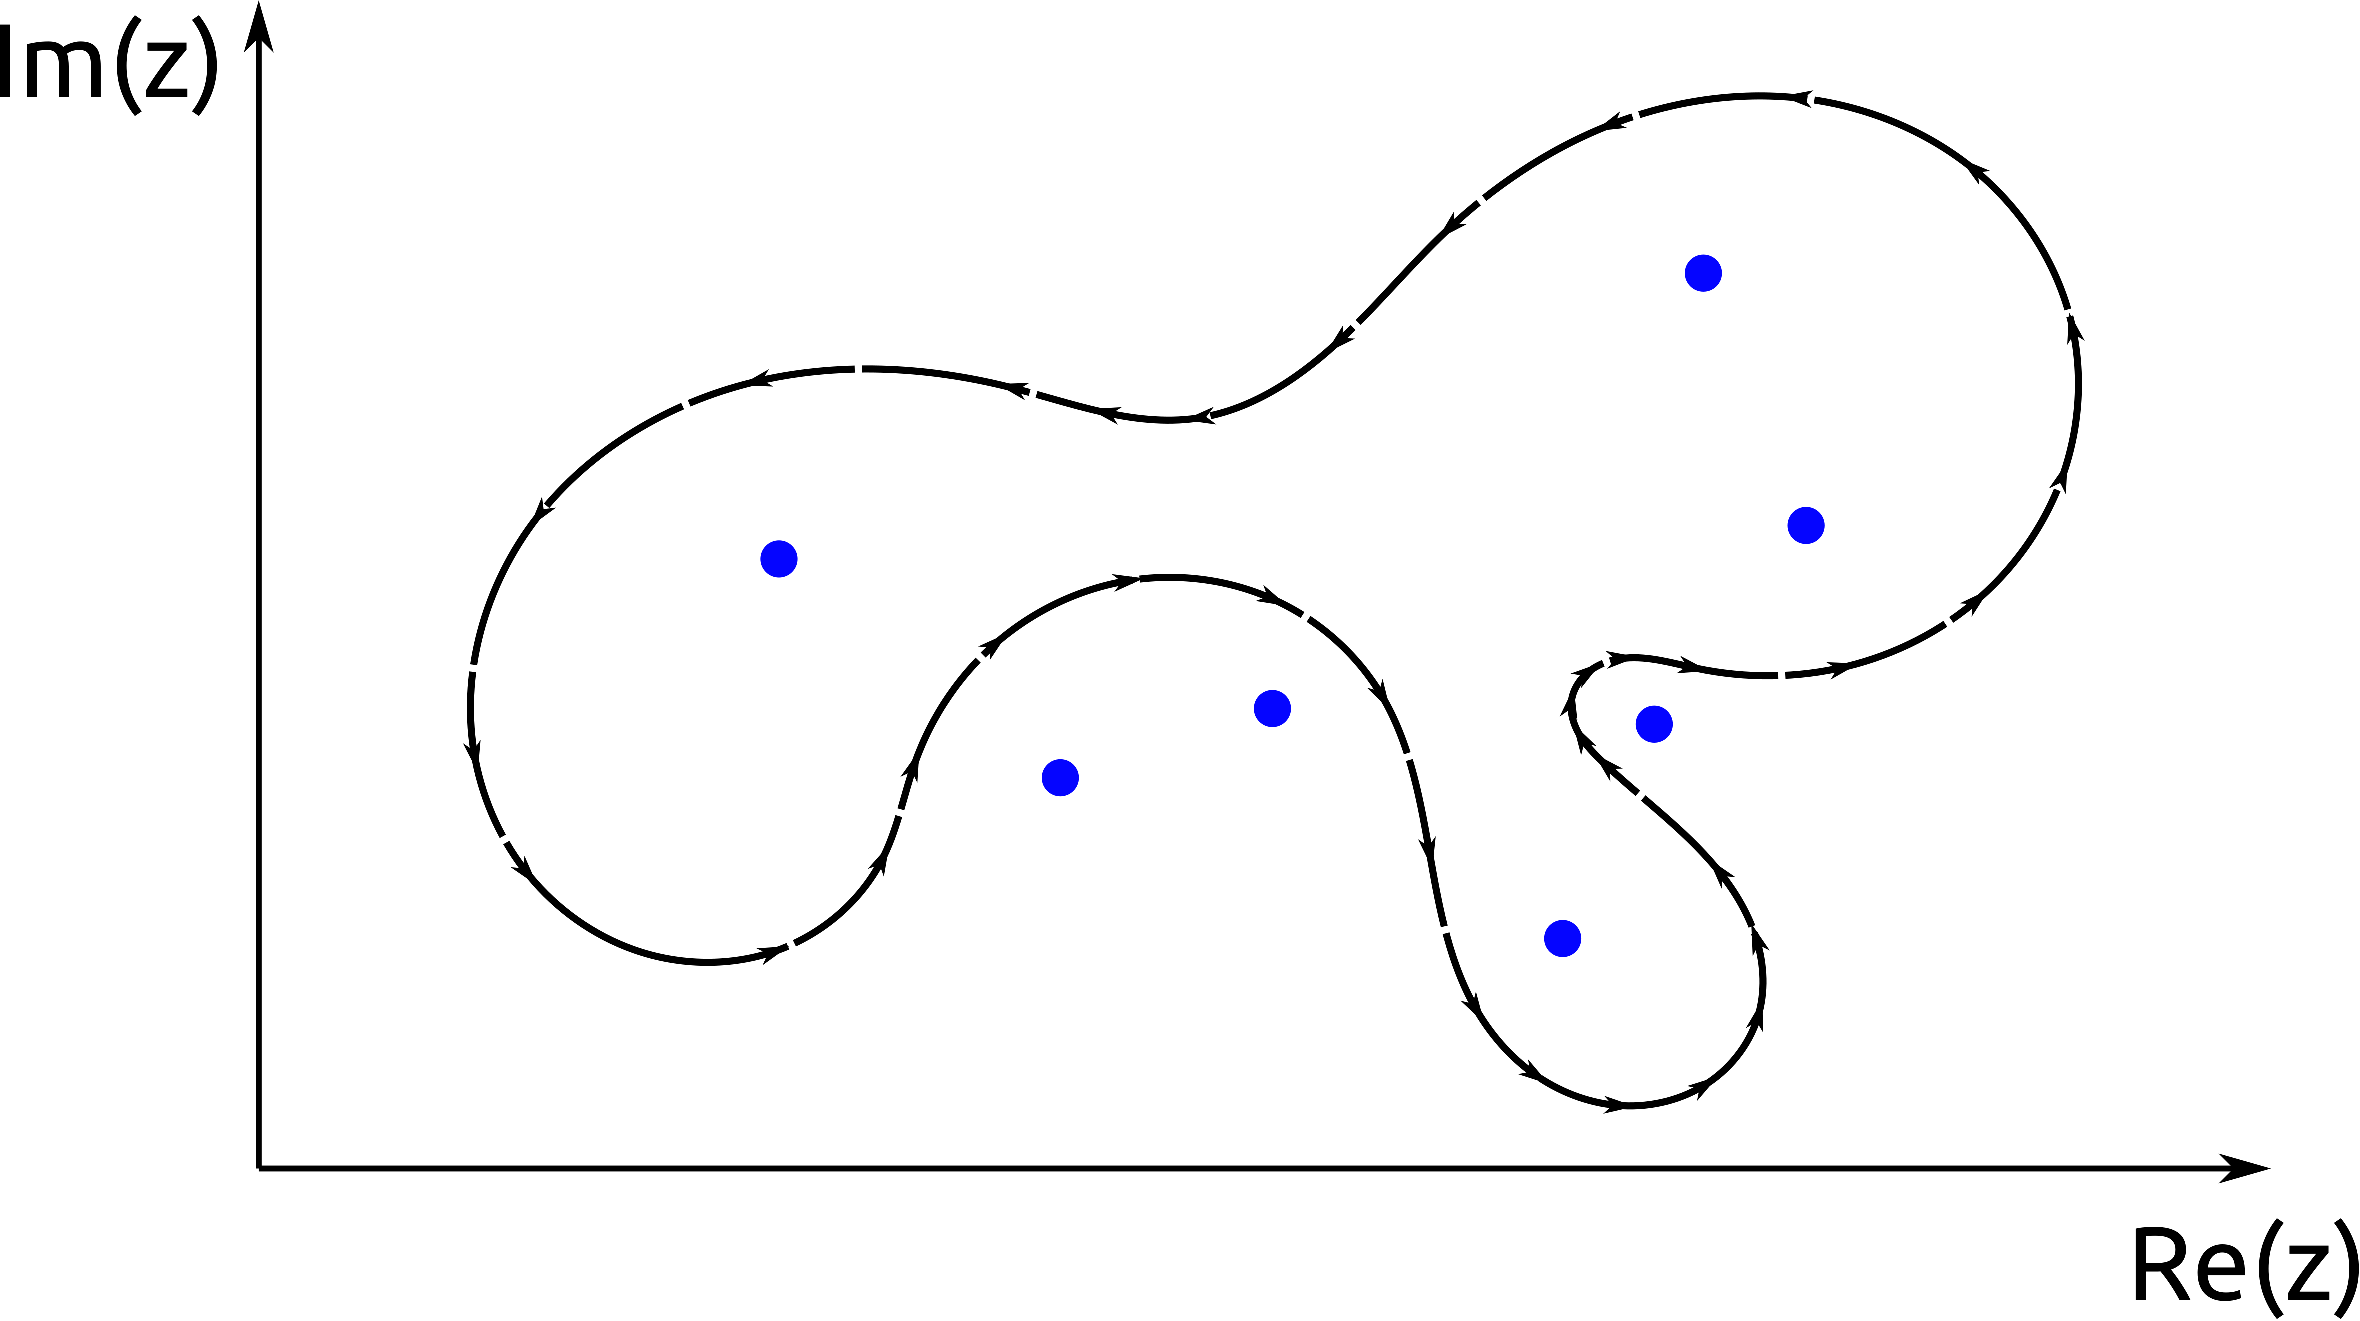
\includegraphics[width=0.5\linewidth]{images/theory/couchy-eps-converted-to.pdf}
%     }
%     \caption{Traversing several zeros on the complex plane.}
%     \label{fig:couchy}
% \end{figure}

% \begin{figure}[tpb]
%     \center{
%         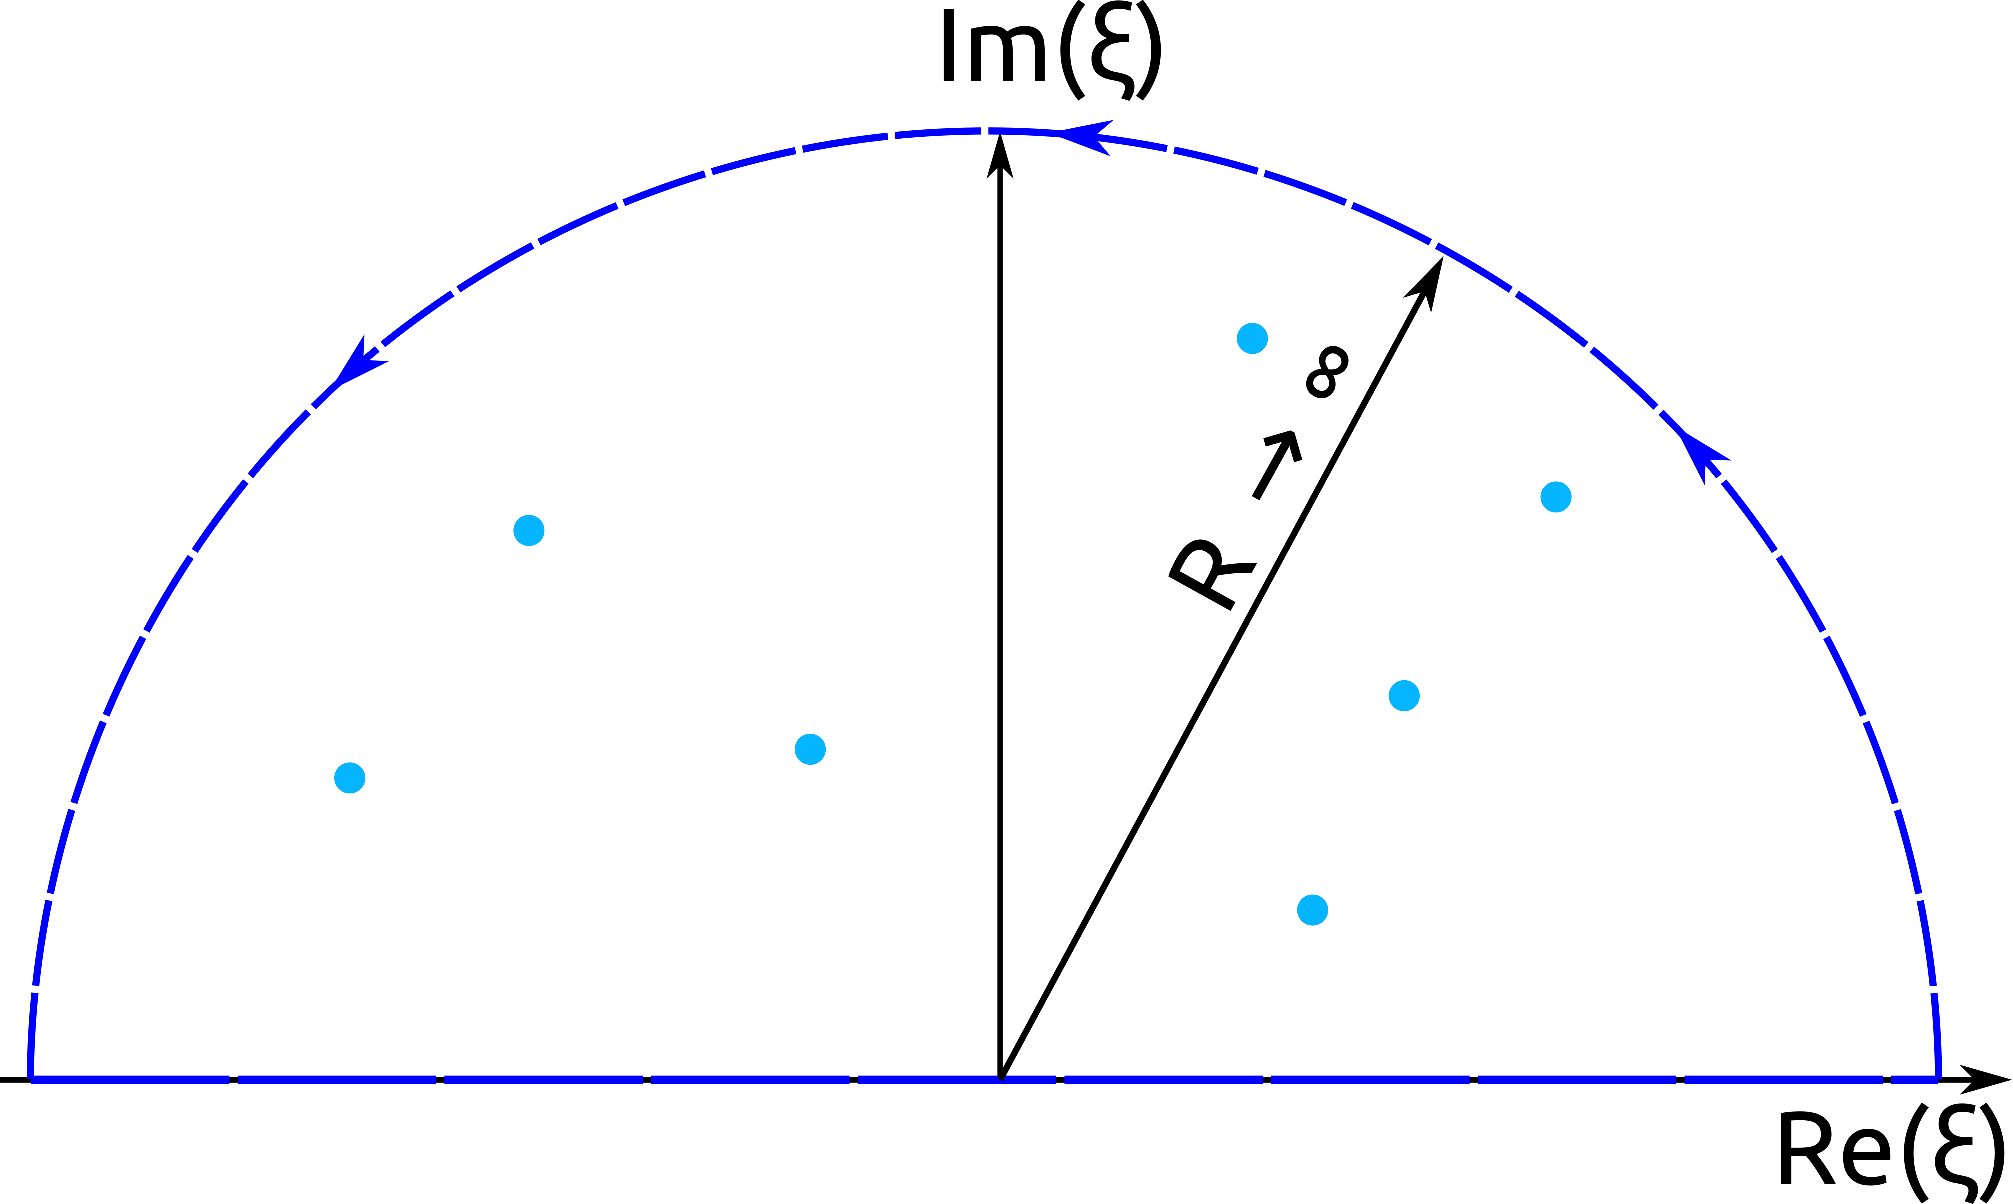
\includegraphics[width=0.5\linewidth]{images/theory/couchy_N-eps-converted-to.pdf}
%     }
%     \caption{Calculate the number of zeros of a complex function.}
%     \label{fig:couchy_N}
% \end{figure}

\begin{figure}[tpb]
    \begin{minipage}[h]{0.5\linewidth}
    \center{
        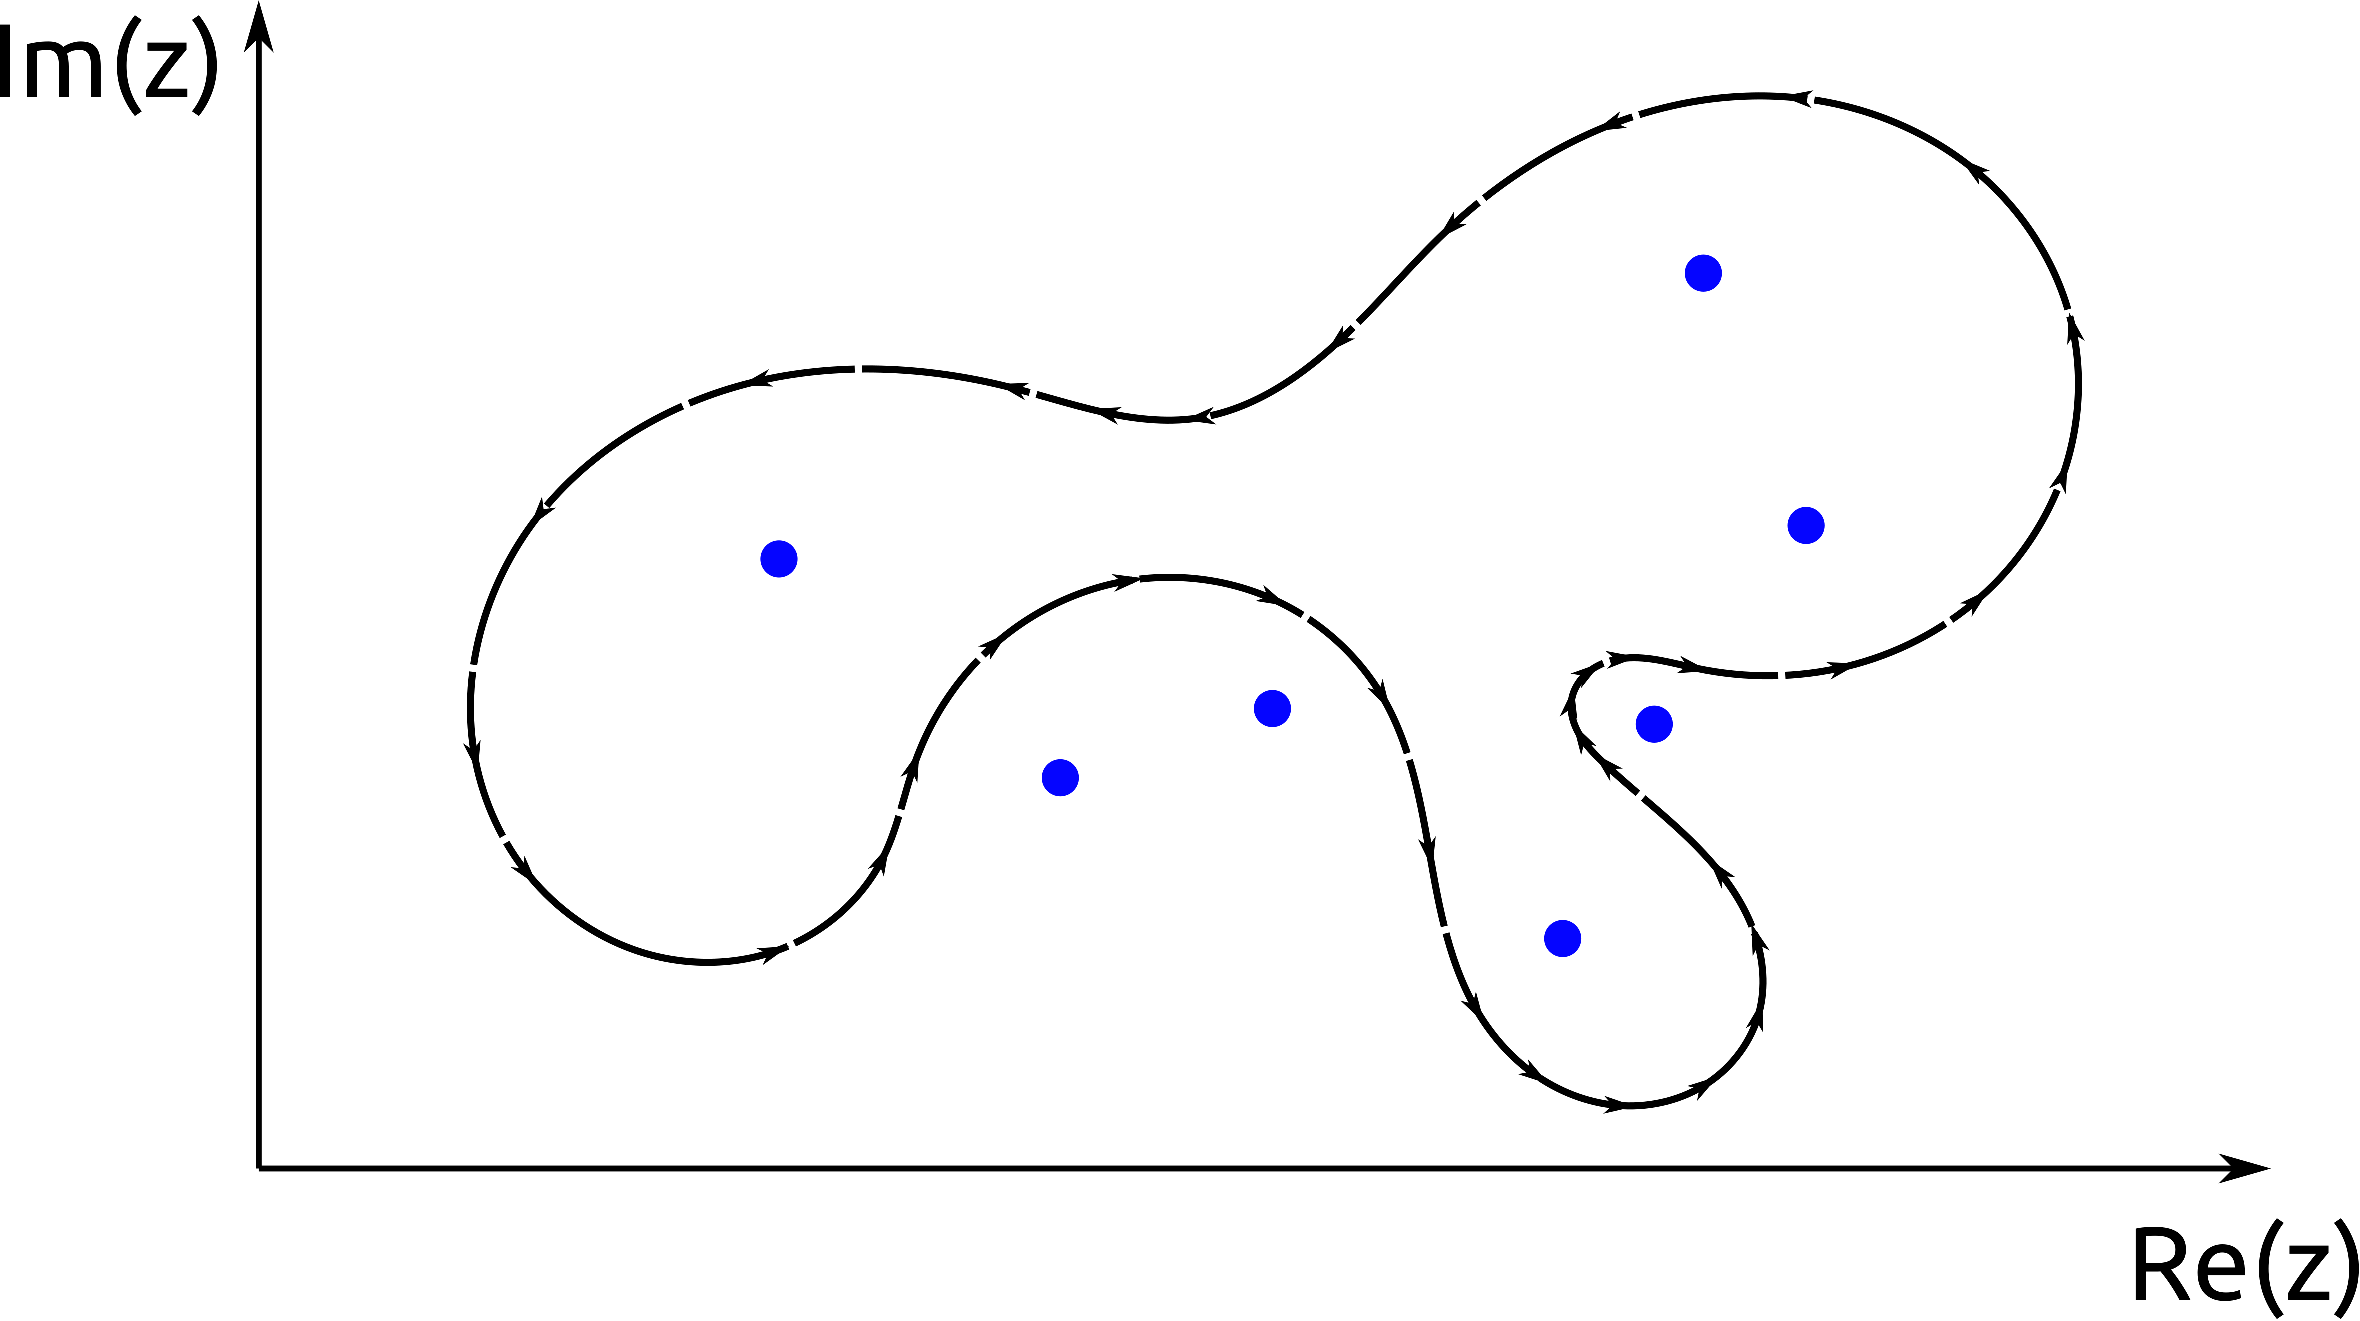
\includegraphics[width=1\linewidth]{images/theory/couchy-eps-converted-to.pdf} (a) \\
    }
    \end{minipage}
    \hfill
    \begin{minipage}[h]{0.46\linewidth}
    \center{
        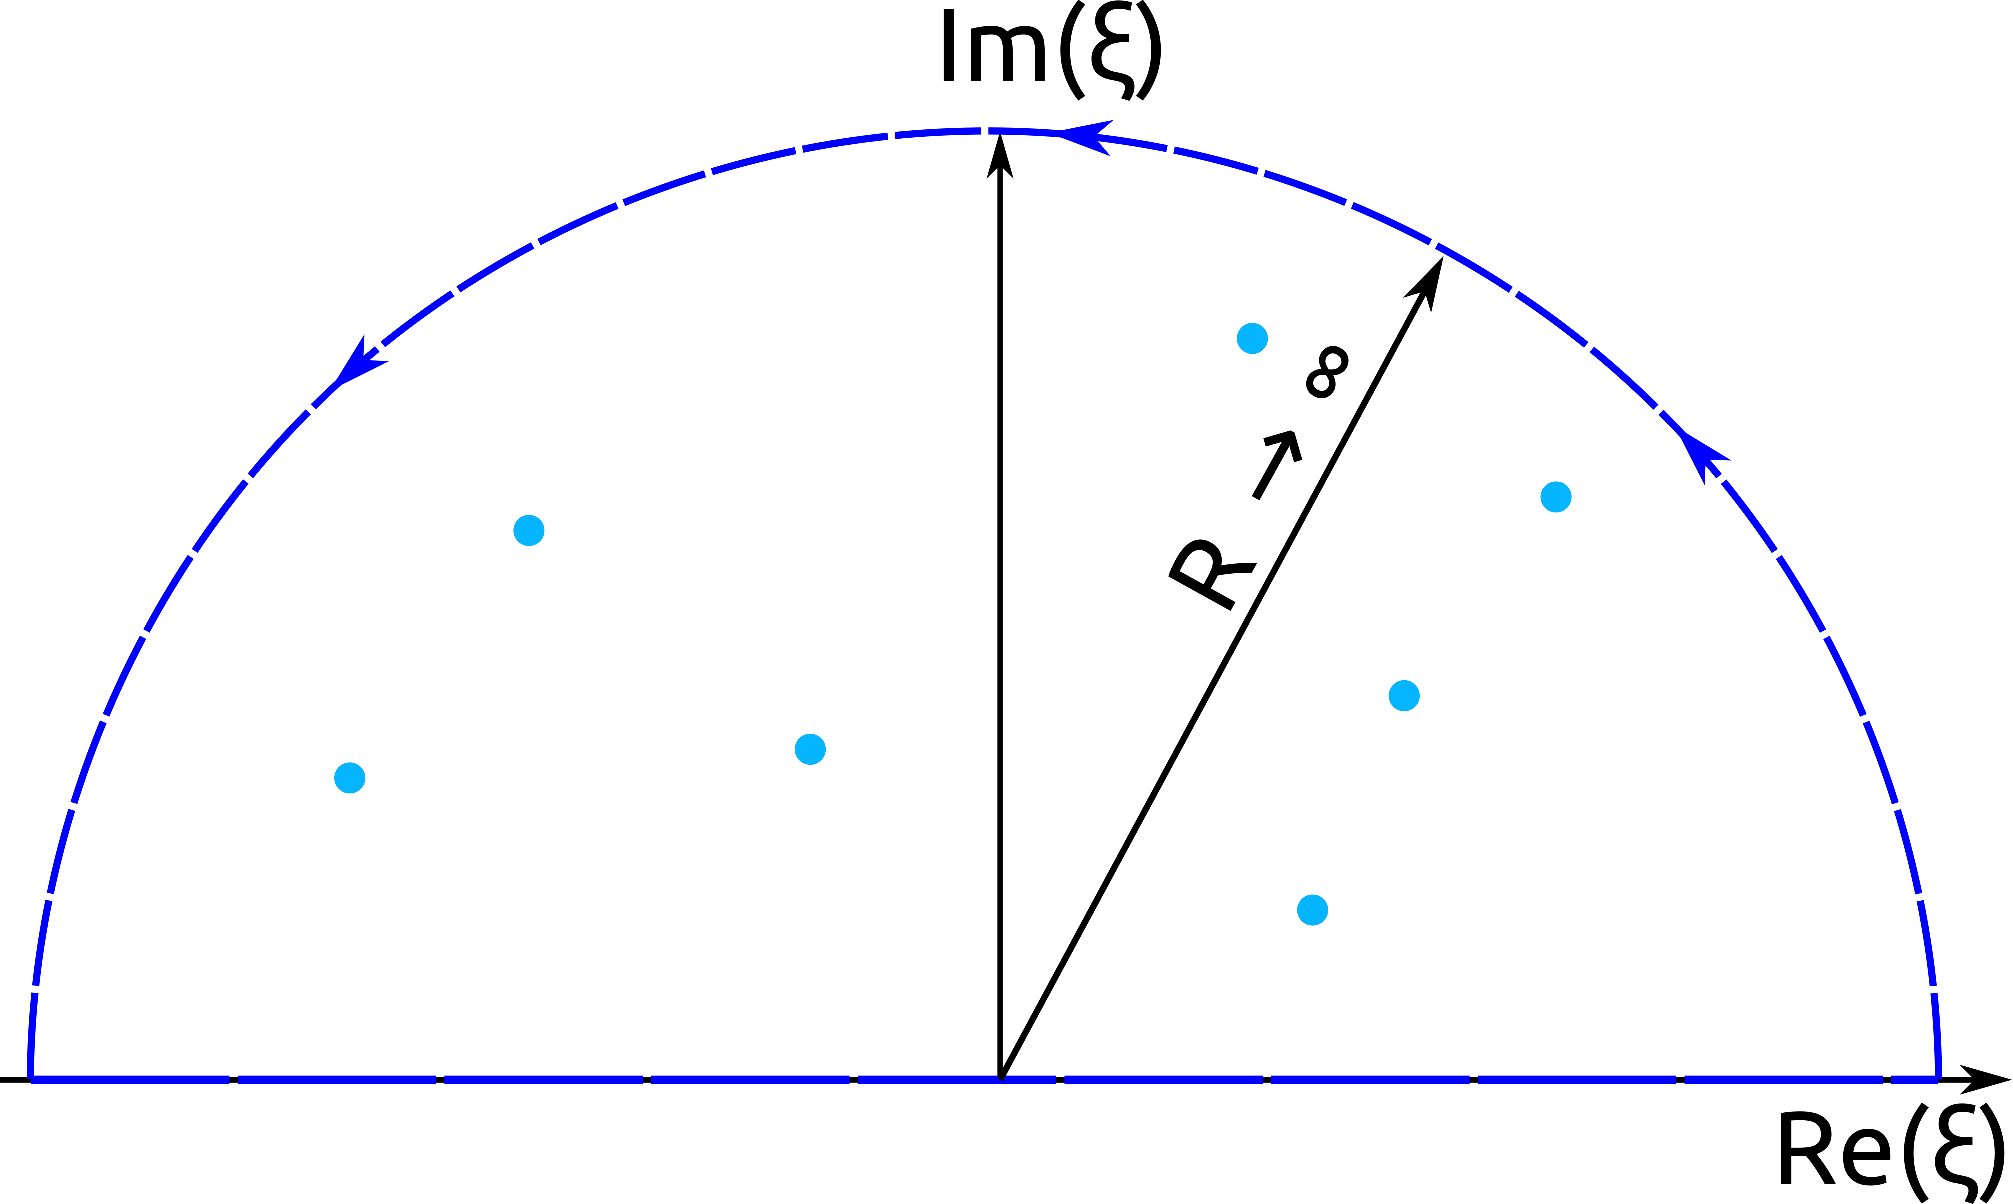
\includegraphics[width=1\linewidth]{images/theory/couchy_N-eps-converted-to.pdf} (b) \\
    }
    \end{minipage}
    \caption{\textbf{(a)} Traversing several zeros on the complex plane. \textbf{(b)} Calculation the number of zeros of a complex function.}
    \label{fig:couchy}
\end{figure}

To find the individual eigenvalues, the so-called Newton identities $ \{\sigma \}_{p = 1}^P $ are used:
\begin{eqnarray}
    - \sum_{j=1}^P \xi_j = \sigma_1 {,} \nonumber \\
    \xi_1 \xi_2 + \xi_2 \xi_3 + ... + \xi_{P-1} \xi_P = \sigma_2 {,} \nonumber \\
    ... \nonumber \\
    (-1)^P \xi_1 \xi_2 ... \xi_P = \sigma_P {.}
\end{eqnarray}
which are associated with the value of the integrals:
\begin{eqnarray}
    s_1 + \sigma_1 = 0 {,} \nonumber \\
    s_2 + s_1 \sigma_1 + 2 \sigma_2 = 0 {,} \nonumber \\
    ... \nonumber \\
    s_P + s_{P-1} \sigma_1 + ... + s_1 \sigma_{P-1} + P \sigma_P = 0 
\end{eqnarray}
%\textbf{откуда появились N}. 
Solving this system, we obtain the values of each Newton identity, calculated by the recurrence formula:
\begin{equation}
    \sigma_p = -\frac{1}{p} \left( s_p + \sum_{j = 1}^{p-1} s_j \sigma_{p-j} \right){,} \quad p = 1...P {.}
\end{equation}

As a result, $ \sigma_p $ (up to a sign) are Viète’s formulas for the polynomial
\begin{equation}
    M(z) = z^P + \sigma_1 z^{P-1} + \sigma_2 z^{P-2} + ... + \sigma_{P-1} z + \sigma_{P} {,}
    \label{eq:m_contour}
\end{equation}
which zeros coincide with the zeros of the original coefficient $ a (\xi) $. Using any algorithm to find the zeros of a polynomial, we thus calculate the discrete spectrum $ \{\xi_j \}_{j = 1}^{P} $.

One of the ways to find the zeros of the polynomial~(\ref{eq:m_contour}) is to go to the problem of finding eigenvalues of the so-called companion matrix $ C (M) $:
\begin{equation}
    C(M(z)) = 
    \begin{bmatrix}
        0 & 0 & \dots & 0 & -\sigma_{P} \\
        1 & 0 & \dots & 0 & -\sigma_{P-1} \\
        0 & 1 & \dots & 0 & -\sigma_{P-2} \\
        \vdots & \vdots & \ddots & \vdots & \vdots \\
        0 & 0 & \dots & 1 & -\sigma_{1} \\
    \end{bmatrix} {,}
\end{equation}
for which the polynomial~(\ref{eq:m_contour}) is a characteristic polynomial.
There exist effective algorithms of finding eigenvalues of such a matrix, for example, the QR-algorithm \cite{kublanovskaya1963, francis1961, francis1962}.

